\documentclass[a4paper,UTF8,fontset=fandol,zihao=-4]{ctexart}
\usepackage[margin=20mm,top=18mm,bottom=18mm]{geometry}
\usepackage{lmodern,amsmath,booktabs,tabularx,graphicx,caption,xcolor,tikz}
\usetikzlibrary{arrows.meta}
\usepackage[unicode,colorlinks]{hyperref}

\definecolor{ink}{HTML}{1B343A}
\definecolor{sea}{HTML}{245F5B}
\hypersetup{
  pdftitle={视觉世界模型驱动的无人艇航行模拟软件开发日志},
  pdfauthor={朱华天、GPT-6.2 Sol},
  linkcolor=sea,urlcolor=sea,citecolor=sea
}
\ctexset{
  section/format=\Large\heiti\color{ink},
  section/beforeskip=0.8\baselineskip,
  section/afterskip=0.42\baselineskip,
  subsection/format=\large\heiti\color{ink},
  subsection/beforeskip=0.55\baselineskip,
  subsection/afterskip=0.25\baselineskip
}
\graphicspath{{images/}}
\captionsetup{font=small,labelfont=bf,skip=5pt,hypcap=false,labelsep=quad}
\setlength{\parskip}{0.28em}
\renewcommand{\arraystretch}{1.16}
\pagestyle{plain}

\newcommand{\voyageframe}[2]{%
  \begin{minipage}[t]{0.475\linewidth}
    \centering
    \includegraphics[width=\linewidth]{#1}\par
    \vspace{2pt}
    {\footnotesize #2\par}
  \end{minipage}%
}

\begin{document}
\begin{center}
  {\heiti\color{ink}\fontsize{20}{27}\selectfont 视觉世界模型驱动的无人艇航行模拟软件开发日志\par}
  \vspace{0.6em}
  {\large 朱华天、GPT-6.2 Sol\par}
  \vspace{0.28em}
  2026年11月18日\par
  {\small\url{https://github.com/ZHT1235456/USV-world-model-demo}\par}
\end{center}

\section{开发目标与实现过程}

本项目在模拟港池中构建了一套由视觉世界模型驱动的无人艇自主航行系统。无人艇需依据海图指定的通行侧别与次序依次绕过彩色航标，探测到临时浮排后择侧避障，并最终减速穿过出场门。交互界面同步展示三维仿真场景、艇载原始前视及实时视觉解析结果。

开发初期先打通了船模、艇载相机与三标航线的最小闭环，随后将核心链路解耦为“视觉状态估计”与“船体动力学”两个可复用模块。选舵流程借鉴了 PlaNet 的范式\cite{hafner2019}，从视觉观测出发，前向推演未来运动，再择优输出动作。此后，系统逐步扩展至浮排避障、低速穿门与反向起航。所有港池共享同一套模型权重，切换场景时通过海图配置航标次序、通行侧与出场门位置。

\begin{center}
  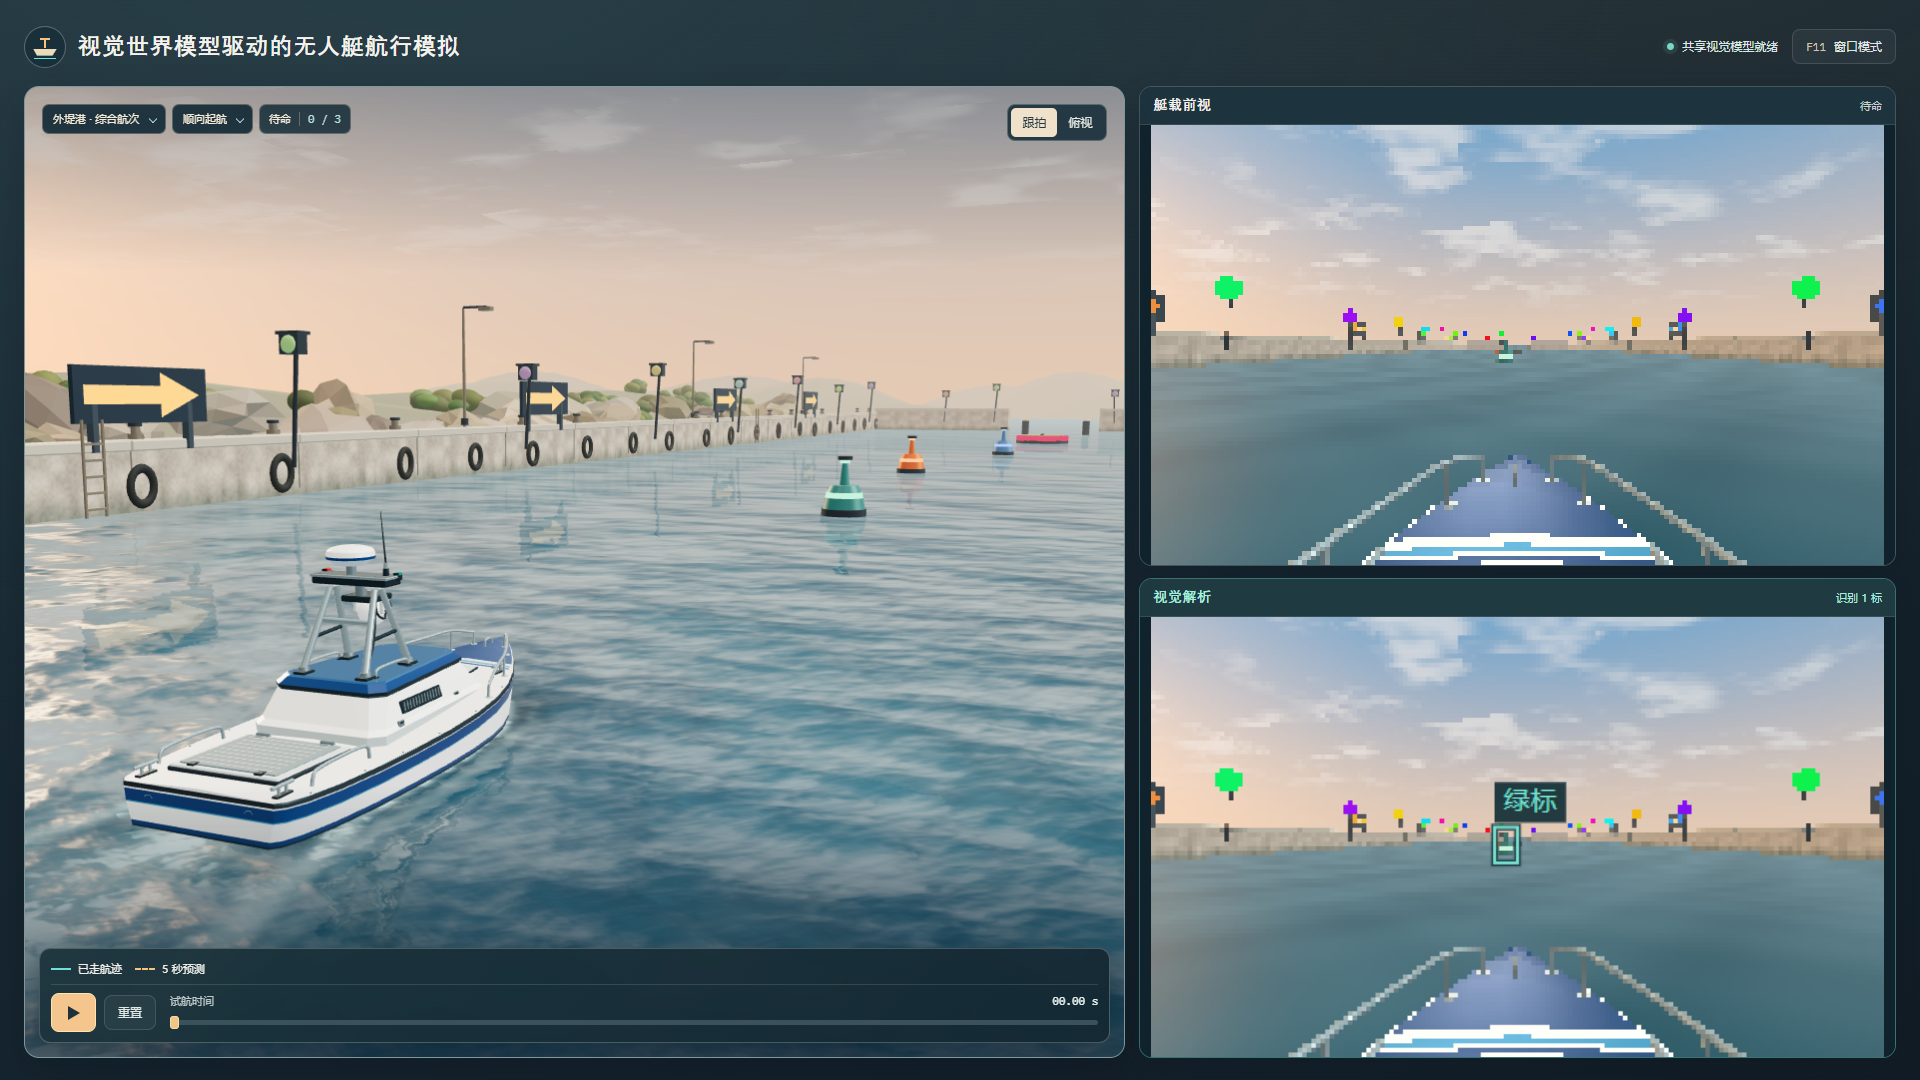
\includegraphics[width=0.92\linewidth,height=64mm,keepaspectratio]{interface.png}
  \captionof{figure}{发布版运行界面。左侧为三维场景，右上为原始前视，右下为同帧视觉解析。}
\end{center}

\section{技术栈}

\noindent\begin{tabularx}{\linewidth}{@{}p{25mm}X@{}}
  \toprule
  模块环节 & 技术实现 \\
  \midrule
  场景与界面 & 基于 Three.js、Vite 与 JavaScript 构建程序化艇模、港池环境及回放界面。\\
  仿真与训练 & 使用 JavaScript 推进船体仿真并采集 RGB 序列，结合 PyTorch 离线拟合视觉估计器与状态转移参数。\\
  推理与部署 & Web Worker 通过 ONNX Runtime Web 执行 WASM 推理。Windows 免安装版由 Tauri 2 和 Rust 封装，界面运行于 WebView2。\\
  \bottomrule
\end{tabularx}

\newpage
\section{世界模型的工作机制}

在线闭环中，世界模型负责将实时视觉观测映射为当前艇况，并推演不同控制指令下的后续运动。该模块由运行在浏览器 Worker 中的两组 ONNX 权重协同实现。

\begin{description}
  \item[状态估计] \texttt{observer.onnx} 融合时序前视画面、光学定位结果与历史指令，输出无人艇当前的位姿与运动速度。
  \item[前向推演] \texttt{motion.onnx} 以当前估计状态为起点，对候选转速与舵角组合迭代预测未来航迹。规划器择优后仅执行首步动作，并在下一轮决策时用新采集的画面刷新状态估计，形成滚动闭环。
\end{description}

反向起航时，系统先依据画面中的黄色箭头定位点解算当前艏向，再并行对比左右掉头轨迹以完成转向决策（见图~\ref{fig:inlet-voyage}（b））。

\begin{center}
  \begin{tikzpicture}[
    block/.style={draw=sea!48,fill=sea!6,rounded corners=2mm,
      text=ink,align=center,text width=28mm,minimum height=13mm,inner sep=2mm},
    note/.style={text=ink,font=\footnotesize,align=center,inner sep=2pt},
    flow/.style={-{Stealth[length=2.4mm,width=1.7mm]},draw=sea,line width=0.7pt},
    training/.style={flow,draw=ink!57}
  ]
    \node[block] (sim) at (0,0) {SeaTrial 仿真与\\Three.js 场景};
    \node[block,fill=ink!5,draw=ink!45,text width=34mm] (train) at (3.3,2.1) {PyTorch 离线训练};
    \node[block,fill=sea!13] (world) at (6.6,0) {浏览器 Worker\\世界模型};
    \node[block,text width=19mm] (plan) at (11.7,0) {滚动规划};

    \draw[training] (sim.north)
      -- node[note,left] {训练帧、指令\\和状态标签} (0,2.1)
      -- (train.west);
    \draw[training] (train.east) -- (6.6,2.1)
      -- node[note,right] {ONNX 权重} (world.north);
    \draw[flow] (sim.east) -- node[note,above] {实时前视帧和\\已发指令} (world.west);
    \draw[flow] (world.east) -- node[note,above] {候选预测航迹} (plan.west);
    \draw[flow] (plan.south) -- (11.7,-1.25)
      -- node[note,below] {本步转速和舵角} (0,-1.25)
      -- (sim.south);
  \end{tikzpicture}
  \captionof{figure}{系统实施方案流程图。离线训练导出 ONNX 权重，在线由 Worker 执行推演和滚动规划。}
  \label{fig:world-model-flow}
\end{center}

\section{感知、推演与控制}

\subsection{视觉定位与目标识别}

前视相机以约 \(10\,\mathrm{Hz}\) 输出 \(160\times96\) 的 RGB 帧。定位模块通过匹配岸标及方向箭头两端的黄色编码，在已知相机内参和海图坐标的条件下，基于针孔相机模型\cite{zhang2000}最小化重投影残差，反推出艇体位置与艏向。

航标、浮排及出场门柱均通过色带的像素连通区域检测，两根门柱同时检出时，解析窗标出终点。针对临时浮排，系统结合色带张角与已知半径估算距离，在短时间内获得至少四次一致观测后才将其纳入规划。

\subsection{视觉时序估计与船体动力学}

视觉估计器将最近 20 帧（约 \(2\,\mathrm{s}\)）下采样至 \(40\times24\)，再用 CNN 编码。GRU 融合图像特征、光学定位结果与历史指令，完成位姿校正及线速度、角速度估计\cite{cho2014}。

动作推演模块围绕纵荡、横荡与艏摇三个自由度组织状态，运动方程参考船舶操纵模型\cite{fossen2021}，并基于仿真轨迹拟合推力、阻尼与转向耦合系数。

\newpage
\subsection{滚动选舵规划}

规划器每 \(0.25\,\mathrm{s}\) 从当前估计状态出发，推演候选动作未来 \(5\,\mathrm{s}\) 的航迹，综合绕标侧别、安全净距、航线偏差与过门速度选定当前转速和舵角。

反向起航阶段，推演时域延长至左右各 \(14\,\mathrm{s}\)，并基于转动后的艇身轮廓校验岸界余量。艇身转过横向后主动减速，朝航道内侧移动后再恢复巡航。

\begin{center}
  \voyageframe{voyage/01-ready.png}{（a）选定内湾港与反向起航}\hfill
  \voyageframe{reverse-start.png}{（b）识别黄色方向箭头并向右掉头}\par\smallskip
  \voyageframe{voyage/03-buoys.png}{（c）通过前两个航标}\hfill
  \voyageframe{voyage/04-avoidance.png}{（d）从浮排右侧绕行}\par\smallskip
  \voyageframe{voyage/05-gate.png}{（e）识别出场门并减速}\hfill
  \voyageframe{voyage/06-finish.png}{（f）通过全部四个航标并完成航次}
  \captionof{figure}{v0.1.0 内湾港反向航次的六个关键节点。全程耗时 \(55.67\,\mathrm{s}\)，最小艇身净距 \(0.59\,\mathrm{m}\)，以 \(0.63\,\mathrm{m/s}\) 过门。解析窗中绿色箭头为识别出的航道方向，金色曲线为规划航迹。三维窗中琥珀色虚线与青色实线分别表示预测轨迹与历史航迹。}
  \label{fig:inlet-voyage}
\end{center}

\newpage
\section{训练与闭环验收}

视觉估计器在五种港池布局下采集了 \(60\) 趟航次进行重训（顺向、反向、侧向起航各 \(20\) 趟），另设 \(15\) 趟验证航次与 \(12\) 趟离线测试航次。外堤港与内湾港均按整座布局留出作为独立测试场景。离线拟合与评分可读取仿真真值。在线闭环期间，控制器逐帧获取 RGB 图像、历史指令和采样时间，换场时加载固定海图。

\noindent\begin{tabularx}{\linewidth}{@{}p{43mm}X@{}}
  \toprule
  验收项目 & 测试结果 \\
  \midrule
  顺向航次 & 三个场景共通过 \(12/12\) 趟。\\
  反向航次 & 三个场景共通过 \(39/39\) 趟。最小岸界净距 \(0.519\,\mathrm{m}\)，首舵前最大艏向误差 \(0.662^\circ\)。\\
  终点识别 & 上述 \(51\) 趟均在穿门前从相机画面识别到终点。\\
  遮蔽箭头对照 & 首舵前艏向误差扩大至 \(178.8^\circ\) 至 \(179.9^\circ\)，内湾港对照航次因触碰岸界终止。\\
  \bottomrule
\end{tabularx}

以上结果来自具备已测绘岸标、可见导航色块与静态浮排的仿真港池。项目源码包含数据采集、训练与闭环评估脚本，并附带运行所需的 ONNX 权重。

Windows x64 免安装版（v0.1.0）为单个约 \(11.56\,\mathrm{MB}\) 的 EXE，内置前端资源、ONNX 权重及 WASM 推理运行时。\href{https://github.com/ZHT1235456/USV-world-model-demo/releases/tag/v0.1.0}{下载发布版}。

\begin{thebibliography}{9}
\small
\bibitem{hafner2019}
Hafner D, Lillicrap T, Fischer I, et al.
Learning Latent Dynamics for Planning from Pixels.
\emph{Proceedings of the 36th International Conference on Machine Learning},
PMLR 97, 2555--2565, 2019.
\href{https://proceedings.mlr.press/v97/hafner19a.html}{PMLR 论文}

\bibitem{zhang2000}
Zhang Z. A Flexible New Technique for Camera Calibration.
\emph{IEEE Transactions on Pattern Analysis and Machine Intelligence},
22(11), 1330--1334, 2000.
\href{https://doi.org/10.1109/34.888718}{DOI 10.1109/34.888718}

\bibitem{cho2014}
Cho K, van Merri\"enboer B, Gulcehre C, et al.
Learning Phrase Representations using RNN Encoder--Decoder for Statistical Machine Translation.
\emph{Proceedings of EMNLP}, 1724--1734, 2014.
\href{https://aclanthology.org/D14-1179/}{ACL Anthology}

\bibitem{fossen2021}
Fossen T I. \emph{Handbook of Marine Craft Hydrodynamics and Motion Control}.
2nd ed., Wiley, 2021.
\href{https://doi.org/10.1002/9781119575016}{DOI 10.1002/9781119575016}
\end{thebibliography}

\end{document}
